\documentclass{standalone}
\usepackage{amsmath}
\usepackage{tikz}
\usepackage{enumitem}
\usetikzlibrary{arrows, shapes, calc, backgrounds, fit, decorations.markings}

\begin{document}

	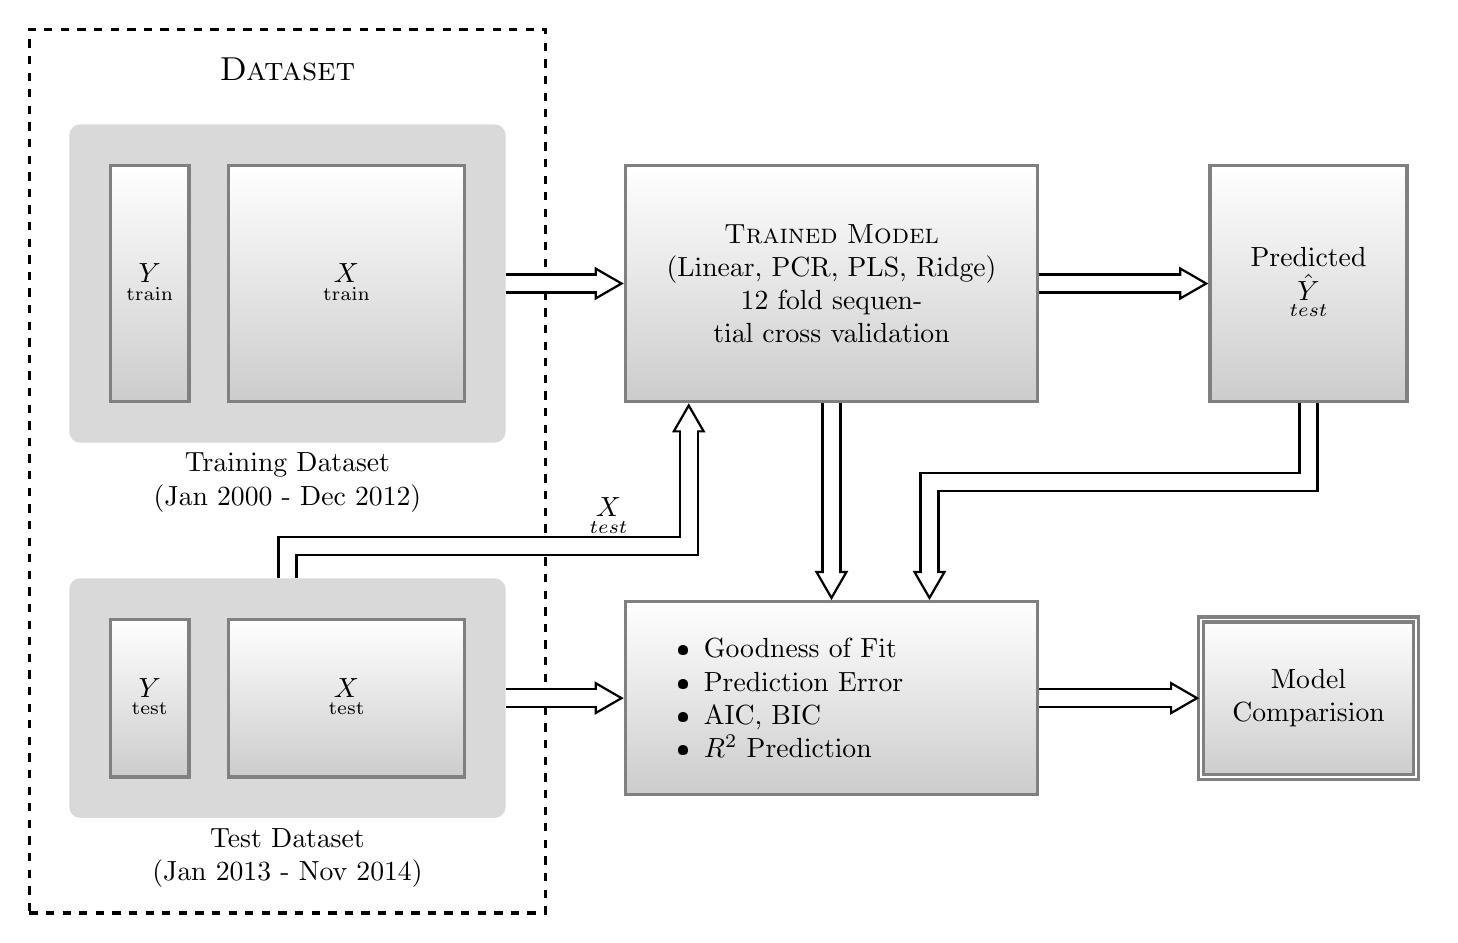
\begin{tikzpicture}[
	every matrix/.style={column sep=2cm,row sep=2.5cm},
	pblock/.style = {rectangle split, rectangle split parts=2, very thick,draw=black!50, top color=white,bottom color=black!20, align=center, minimum height=3cm},
	block/.style = {rectangle,very thick,draw=black!50, top color=white, bottom color=black!20, align=center, minimum height=#1},
	myarrow/.style = {double, double distance=2mm, thick, shorten >= 10.5pt, decoration={markings,mark=at position 1 with {\arrow[scale=2,thin]{open triangle 60}}},
	preaction={decorate},
	postaction={draw,line width=2mm, white,shorten >= 9.5pt},
	},                   
	]
		\matrix{
			\node[block={3cm}, minimum width =1cm] (Ytrain) {$\underset{\text{train}}{Y}$};
			\node[block={3cm}, right of = Ytrain, node distance=2.5cm, minimum width=3cm](Xtrain){$\underset{\text{train}}{X}$}; &
			\node[block={3cm}, minimum width=5cm, align=center, text width=5cm](trainedModel){\textsc{Trained Model} \\
			(Linear, PCR, PLS, Ridge) \\ 12 fold sequential cross validation}; &
			\node[block={3cm}, minimum width=2.5cm, align=center](predY){Predicted \\ $\underset{test}{\hat{Y}}$};\\
			
			\node[block={2cm}, minimum width =1cm] (Ytest) {$\underset{\text{test}}{Y}$};
			\node[block={2cm}, right of = Ytest, node distance=2.5cm, minimum width=3cm, align=center](Xtest){$\underset{\text{test}}{X}$}; &
			\node[block={2cm}, minimum width=5cm](compCriteria){
			\parbox{5cm}{\begin{itemize}[noitemsep]
						\item Goodness of Fit
						\item Prediction Error 
						\item AIC, BIC 
						\item $R^2$ Prediction
						\end{itemize}}}; &
			\node[block={2cm}, minimum width=2.5cm, text width=2.5cm, align=center, double](Final){Model \\Comparision};\\
		};
		
	\begin{scope}[on background layer]
	   \node(trainSet) [fit=(Ytrain) (Xtrain), fill= gray!30, rounded corners, inner sep=.5cm, label={[align=center]below:Training Dataset\\(Jan 2000 - Dec 2012)}] {};
	   \node(testSet) [fit=(Ytest) (Xtest), fill= gray!30, rounded corners, inner sep=.5cm, label={[align=center]below:Test Dataset\\(Jan 2013 - Nov 2014)}] {};
        \node(dataSet) [fit=(trainSet) (testSet), inner ysep=1.2cm, inner xsep=0.5cm, rectangle, very thick, dashed, draw, label={[yshift=-0.8cm]\large\textsc{Dataset}}] {};
	 \end{scope}
		
		\draw[myarrow](trainSet) -- (trainedModel);
		\draw[myarrow](trainedModel) -- (predY);
		\draw[myarrow](trainedModel) -- (compCriteria);
		\draw[myarrow](predY.south) -- +(0, -1cm) -| (compCriteria.45);
		\draw[myarrow](testSet.north) -- +(0, 4mm) -| node[pos=0.4, above]{$\underset{test}{X}$}(trainedModel.220);
		\draw[myarrow](testSet) -- (compCriteria);
		\draw[myarrow](compCriteria) -- (Final);
				
		
	\end{tikzpicture}
\end{document}